\begin{figure}[H]
	\centering
	\caption{Steady State $ k^{*} $ at $ c_{t} = c^{*} $}
	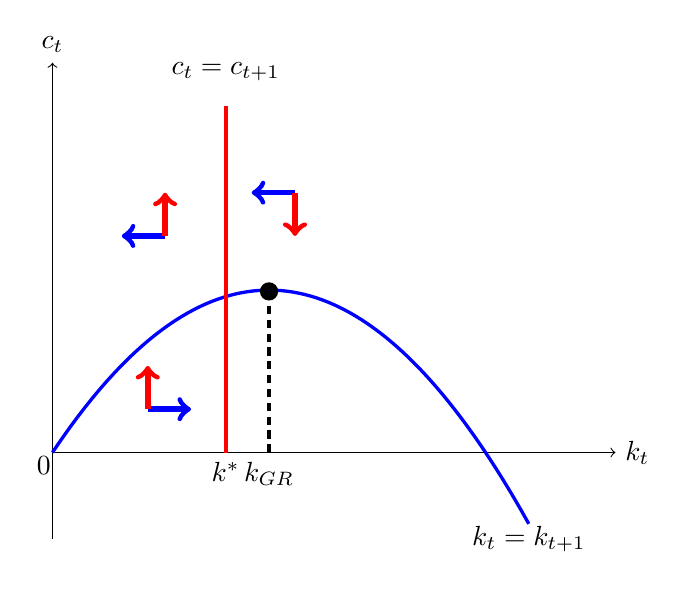
\begin{tikzpicture}[scale=1.1]
		\draw[->] (0, 0) -- (6.5, 0) node[right] {$k_{t}$};
		\draw[->] (0, -1) -- (0, 4.5) node[above] {$c_{t}$};
		\draw[domain=0:5.5, samples=200, blue, line width = 1.2pt, variable=\x] plot ({\x}, {-0.3*\x*(\x-5)});
		\draw[red, line width=1.5pt] (2,0) -- (2,4);
		\node at (-0.1,-0.15) {$0$};
		\node at (5.5,-1) {$ k_{t} = k_{t+1} $};
		\draw[->, blue, line width=2pt] (1.1,0.5) -- (1.6,0.5);
		%\draw[->, blue, line width=2pt] (2.6,1) -- (3.1,1);
		\draw[->, blue, line width=2pt] (2.8,3) -- (2.3,3);
		\draw[->, blue, line width=2pt] (1.3,2.5) -- (0.8,2.5);
		\node at (2,4.4) {$c_{t} = c_{t+1}$};
		\node[below] at (2,0) {$k^*$};
		\draw[->, red, line width=2pt] (2.8,3) -- (2.8,2.5);
		%\draw[->, red, line width=2pt] (2.6,1) -- (2.6,0.5);
		\draw[->, red, line width=2pt] (1.3,2.5) -- (1.3,3);
		\draw[->, red, line width=2pt] (1.1,0.5) -- (1.1,1);
		\node[below] at(2.5,0) {$ k_{GR} $};
		\draw[densely dashed, line width=1.5pt] (2.5,0) -- (2.5,1.86);
		\fill[black] (2.5,1.86) circle (3pt);
	\end{tikzpicture}
\end{figure}
